\chapter{ASIC Implementation}

The VLSI design flow can be divided into two parts
\begin{itemize}
  \itemsep0em 
\item Frontend design flow
    \begin{itemize}
      \itemsep0em 
    \item RTL Design/Coding
	\item Synthesis
	\item Fuctional Verificaion
	\item DFT
    \end{itemize}
\item Backend design flow.
    \begin{itemize}
    \itemsep0em 
    \item Floor Planning
	\item Placement
	\item Clock Tree Synthesis
	\item Routing
	\item Static timing analysis 
	\item Physical Verification
    \end{itemize}
\end{itemize}
Both together allow the creation of a functional chip from scratch to production.
%https://paginas.fe.up.pt/~ee07306/wp-content/uploads/2013/03/desing_flow_LuisGomes_v1.pdf
%https://chipedge.com/company_news/how-to-choose-frontend-vs-backend/

\begin{figure}
  \centering
  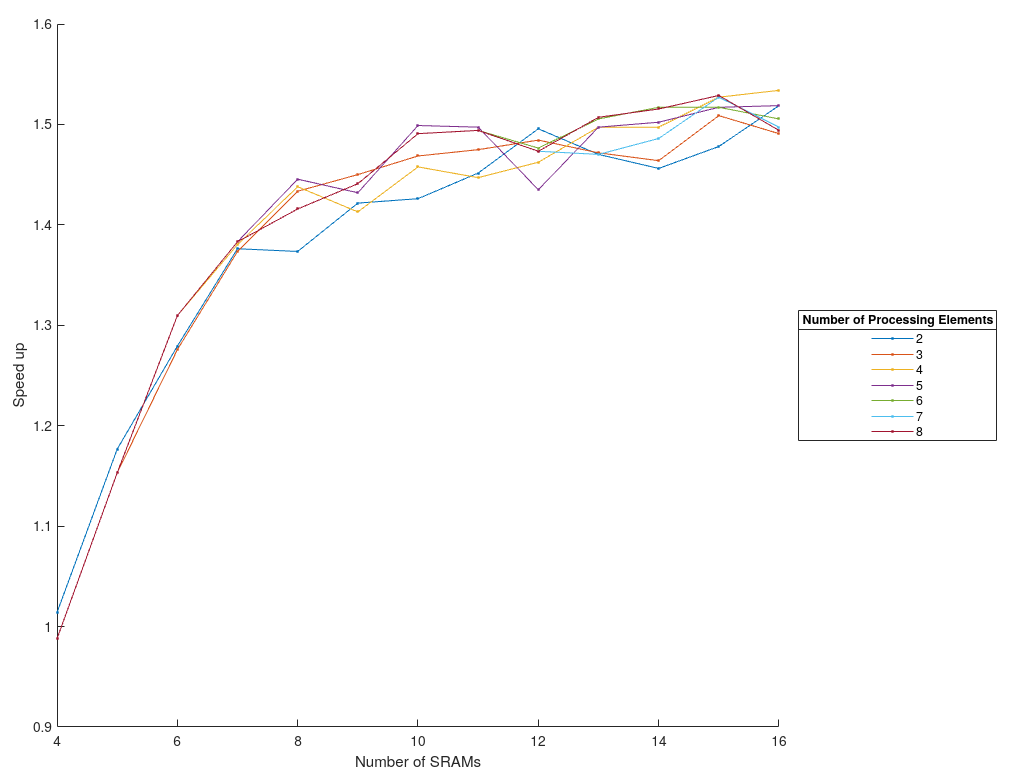
\includegraphics[width=0.5\linewidth]{./ASIC/SRAMvsSpeedup.png}
  \caption{Speed up of Design vs Number of SRAM with varying Processing Element}
\end{figure}

There is a need to analyze the accelerator for optimum use of Hardware. The Optimum value would be 8 SRAM and 4 Processing Elements as per the graph.

Following is the target specification:-
\begin{itemize}
\itemsep0em 
\item Number of Data RAM:- 8
\item Size of Each Data SRAM:- 8 kbits ( width 32-bit depth 256)
\item Size of Instruction SRAM required:-410 kbits ( width 205-bit depth 2048)
\item Number of Processing Elements:- 4 ( 4 MAC and 4 DIV units)
\item Targetted Frequency:- 40 MHz
\end{itemize}
OpenRAM\cite{OpenRAM} will create the SRAM, and OpenLane\cite{OpenLane} RTL to GDS converter will process the design elements. Final Integration will be using Cadence SoC Encounter. The design will be implemented using The Skywater 130nm PDK. This PDK doesn't have support for Propriorty software, although a GitLab configure file helped for Integration\cite{skyADK}.

\section{OpenRAM}

OpenRAM\cite{OpenRAM} is an open-source Python framework for creating the layout, netlists, timing, and power models. It is a Memory Compiler and is used for creating SRAMas macro. This SRAM is used to store Instructions and Matrix Data. Some Common configure files that need to Provide like Supply voltages, Temperature, Process corner, and Number of Ports.
The Output Files includes followings:-
\begin{itemize}
  \itemsep0em 
\item GDS (.gds)
\item SPICE (.sp)
\item Verilog (.v)
\item PnR Abstract (.lef)
\item Liberty (multiple corners .lib)
\item Datasheet (.html)
\item Log (.log)
\item Configuration (.py) for replication of creation
\end{itemize}
Datasheet for Data SRAM and Instructions is Given in Below :-
  \begin{figure}
  \centering
  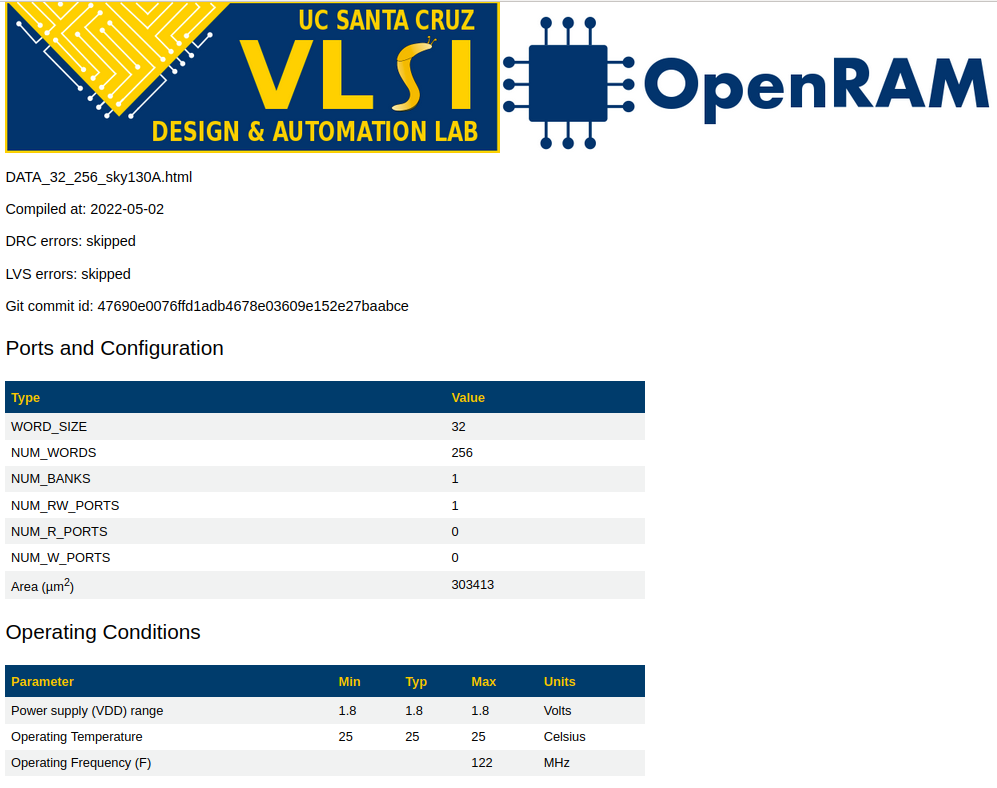
\includegraphics[width=0.8\linewidth]{./ASIC/OpenRAM_Condition.png}
  \caption{OpenRAM Condition for Data SRAM}
  \end{figure}

  \begin{figure}
    \begin{subfigure}{.5\textwidth}
      \centering
      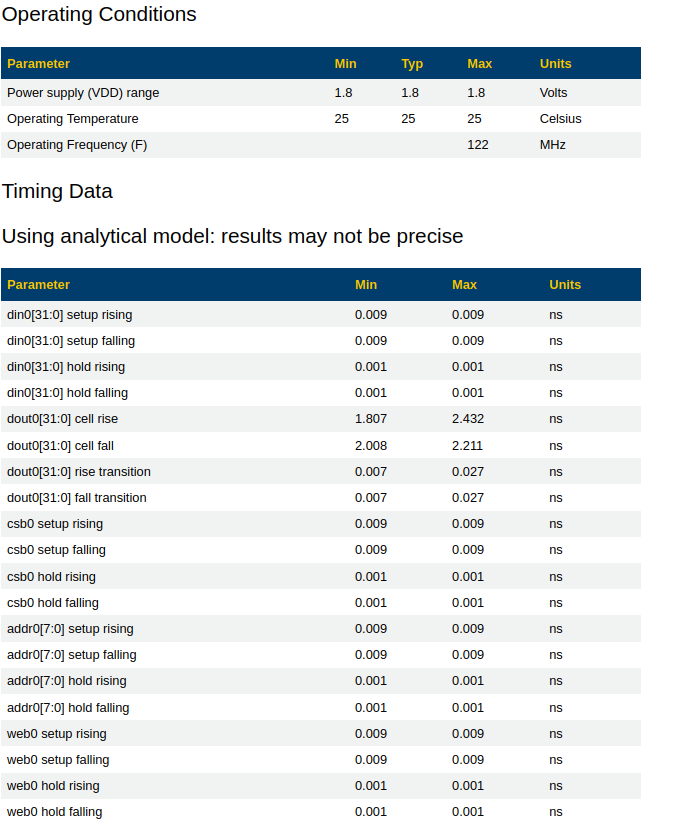
\includegraphics[width=.8\linewidth]{./ASIC/OpenRAM_Timing.png}
      \caption{OpenRAM Timing details}
    %	\label{fig:sfig1}
      \end{subfigure}%
      \begin{subfigure}{.5\textwidth}
      \centering
      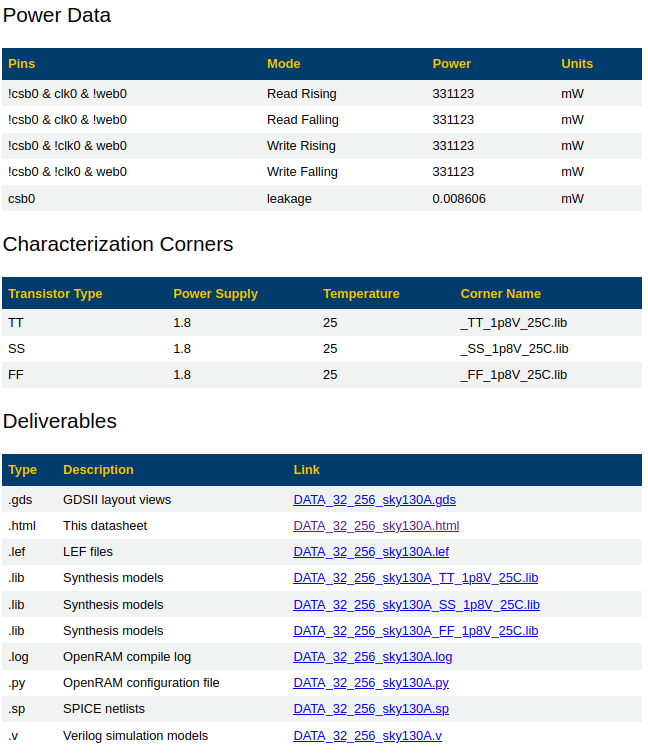
\includegraphics[width=.8\linewidth]{./ASIC/OpenRAM_otherDescription.png}
      \caption{OpenRAM Characteristic and Power details}
    %	\label{fig:sfig2}
      \end{subfigure}
      \caption{OpenRAM Analysis report for Data SRAM}
    %  \label{fig:fig}
    \end{figure}

\begin{figure}
    \centering
    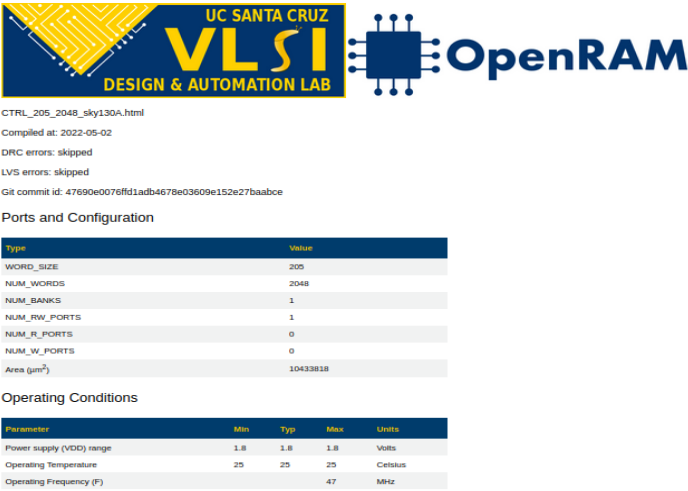
\includegraphics[width=0.8\linewidth]{./ASIC/OpenRAM_INST_condition.png}
    \caption{OpenRAM Condition for Instruction SRAM}
    \end{figure}
  
    \begin{figure}
      \begin{subfigure}{.5\textwidth}
        \centering
        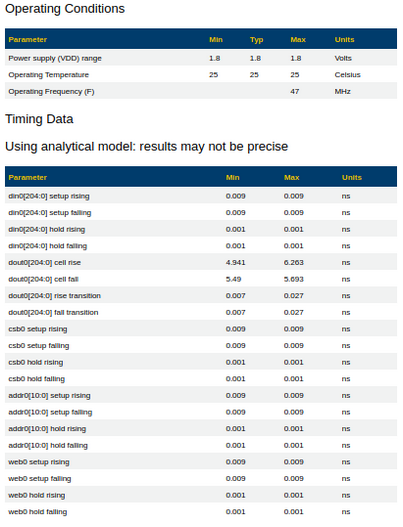
\includegraphics[width=.8\linewidth]{./ASIC/OpenRAM_INST_timing.png}
        \caption{OpenRAM Timing details}
      %	\label{fig:sfig1}
        \end{subfigure}%
        \begin{subfigure}{.5\textwidth}
        \centering
        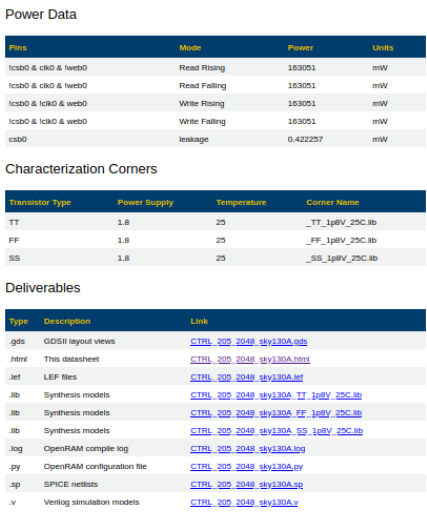
\includegraphics[width=.8\linewidth]{./ASIC/OpenRAM_INST_power.png}
        \caption{OpenRAM Characteristic and Power details}
      %	\label{fig:sfig2}
        \end{subfigure}
        \caption{OpenRAM Analysis report for Instruction SRAM}
      %  \label{fig:fig}
\end{figure}
      
\break

For using the OpenRAM Memory compiler, the following is the directory structure along with specified distinctive attributes.\\
\\
\begin{forest}
    for tree={
      font=\ttfamily,
      grow'=0,
      child anchor=west,
      parent anchor=south,
      anchor=west,
      calign=first,
      edge path={
        \noexpand\path [draw, \forestoption{edge}]
        (!u.south west) +(7.5pt,0) |- node[fill,inner sep=1.25pt] {} (.child anchor)\forestoption{edge label};
      },
      before typesetting nodes={
        if n=1
          {insert before={[,phantom]}}
          {}
      },
      fit=band,
      before computing xy={l=15pt},
    }
  [techname\/
    [\_\_init\_\_.py : Sets up PDK environment]
    [tech : Contains technology configuration
        [\_\_init\_\_.py : Loads all modules]
        [tech.py : SPICE\, DRC\, GDS\, and layer config]
    ]
    [gds\_lib : Contains .gds files for each lib cell]
    [sp\_lib : Contains .sp file for each lib cell]
    [models : Contains SPICE device corner models]
    [tf : May contain some PDK material]
    [mag\_lib : May contain other layout formats]
  ]
\end{forest}

These files should have 
\begin{itemize}
\item Bitcell (and dummy and replica bitcell)
\item Sense amplifier
\item DFF (from a standard cell library)
\item write driver
\end{itemize}

VSD Corp. Pvt. Ltd \cite{VSD} had to share the Technology files of SKYWater 130nm PDK to create OpenRAM. The Macro provided is used for the creation of Physical implementation of the design. The files have an outdated version of Skywater PDK rules for DRC and LVS. Therefore the OpenRAM could produce a design with DRC faults.As per the analysis report, the bottleneck of our design will be Instruction  SRAM, which can run at the maximum frequency of 47 MHz.

\section{OpenLANE}

OpenLANE\cite{OpenLane} is an automated RTL to GDSII flow based. The components include open-source tools, which include followings:-
\begin{itemize}
  \itemsep0em 
    \item YosysHQ
    \item OpenROAD
    \item Open Circuit Design
%    \item CU-GR
%    \item TritonRoute
%    \item DEF2SPEF
%    \item Magic
%    \item Netgen
%    \item CVC
%    \item Klayout
\end{itemize}
\begin{figure}[h]
    \centering
    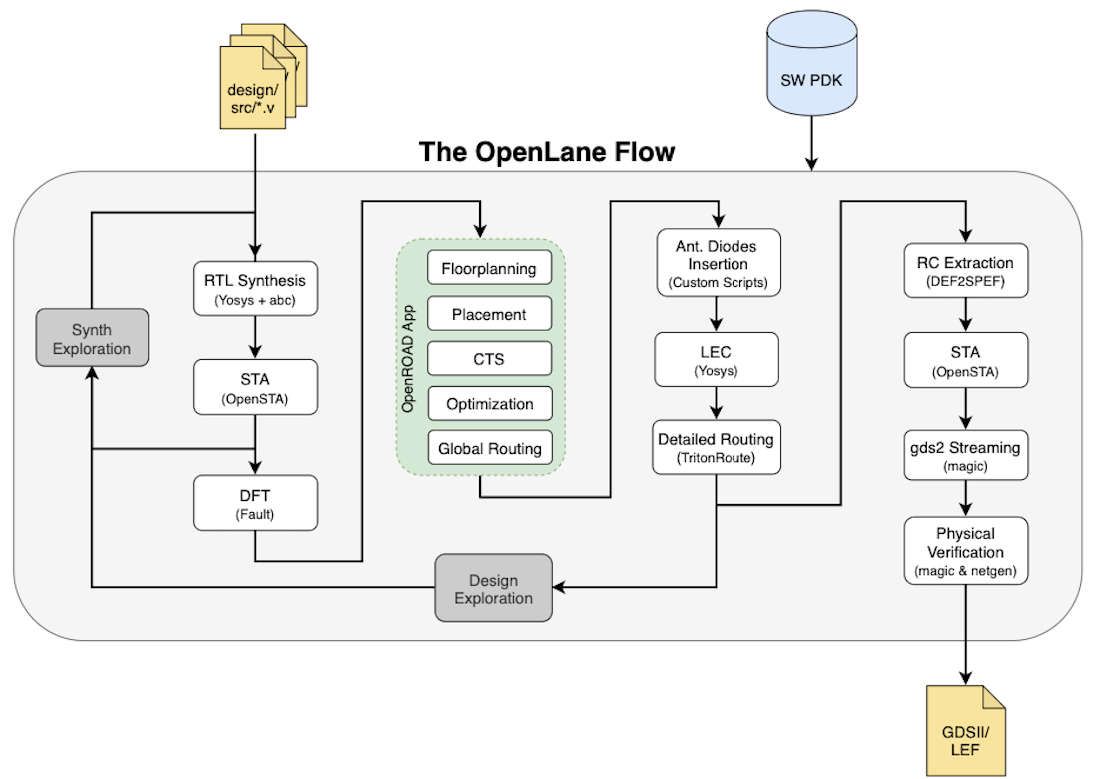
\includegraphics[width = 0.8\linewidth]{./ASIC/openlane_flow.png}
    \caption{OpenLane Flow}
    %\label{fig:Intro:flow}
\end{figure}

The MAC unit has a 9(multiplication) latency +7(Addition)=16 clocks. It is 
cascading of simple floating-point multiplication and addition units of the design. The Division module has a latency of 36 clocks. It includes the restoring division method.

The design was converted from RTL to GDS using OpenLane.Processing elements, i.e., pipelined version of Fused Multuiplicnation Unit and DIV unit, are created using the OpenLane.based on Synth Exploration feature. Design Synthesis Exploration performed the design more importance given to Performance over the area. 

\begin{figure}
\begin{subfigure}{.5\textwidth}
	\centering
	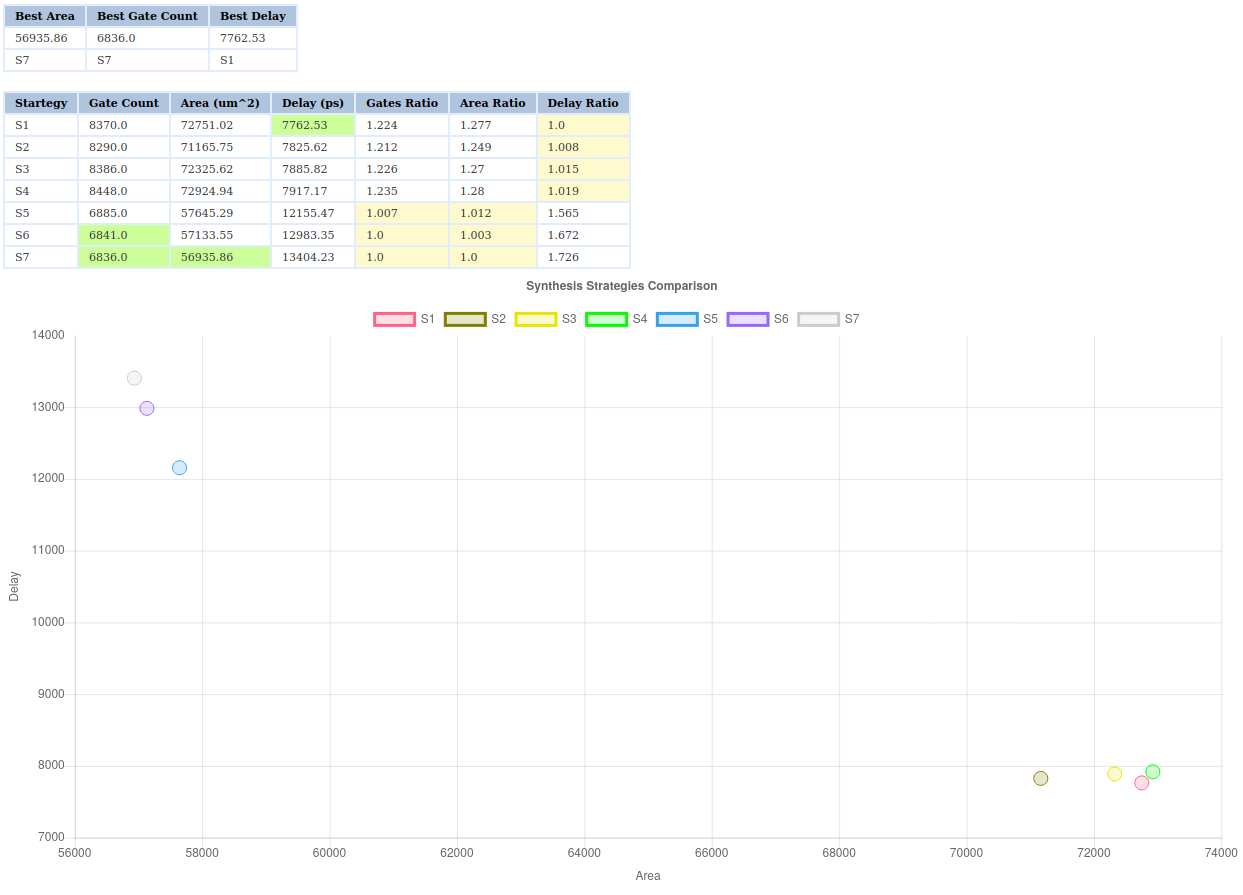
\includegraphics[width=.8\linewidth]{./ASIC/MAC.png}
	\caption{Fused Multiplication Add Unit}
%	\label{fig:sfig1}
  \end{subfigure}%
  \begin{subfigure}{.5\textwidth}
	\centering
	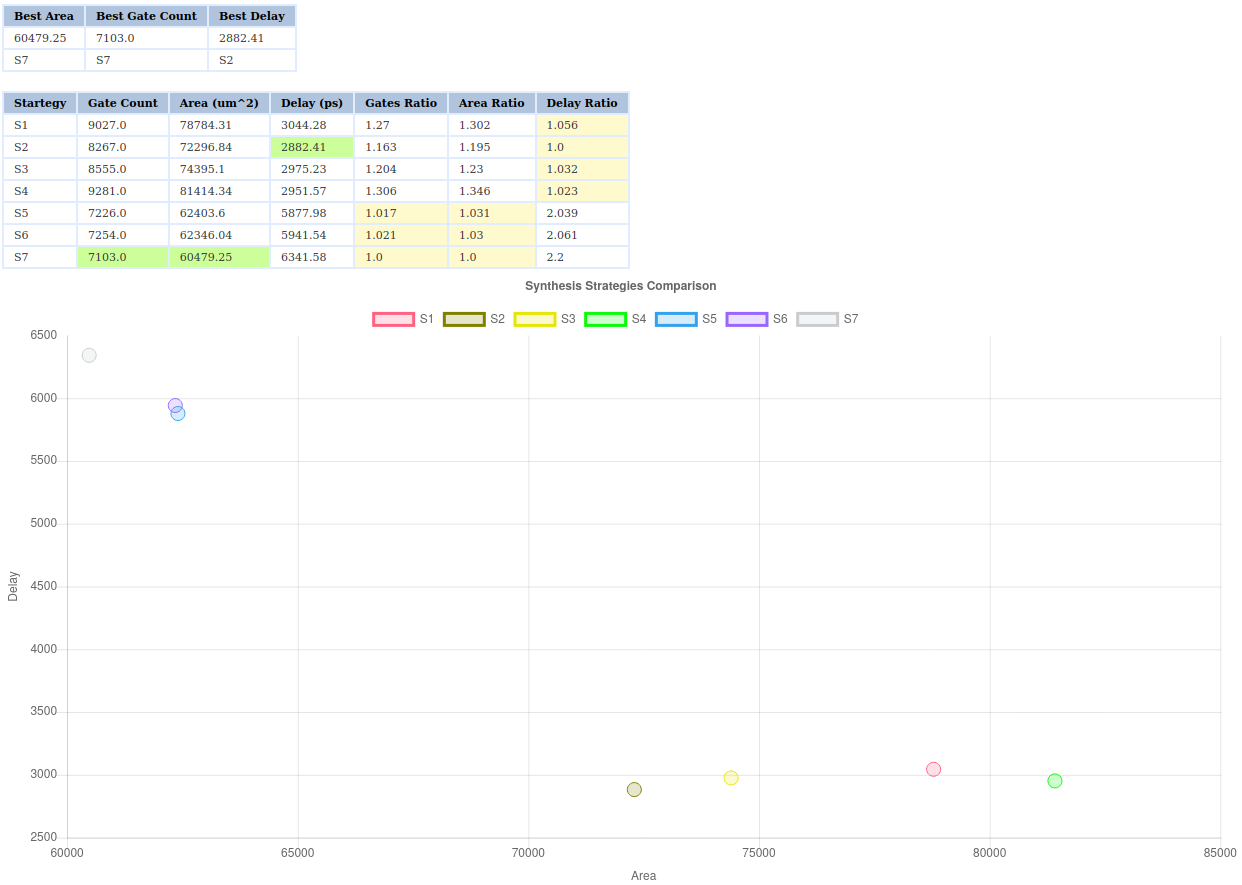
\includegraphics[width=.8\linewidth]{./ASIC/DIV.png}
	\caption{Division Unit}
%	\label{fig:sfig2}
  \end{subfigure}
  \caption{Processing Element Synthesis Analysis Report}
%  \label{fig:fig}
\end{figure}

OpenLANE indeed is a good package for automated RTL to GDS. Although it had the following issues:-
\begin{itemize}
  \itemsep0em
  \item It was not able to give process antenna clean for every design.
  \item Hardening macro is not robust enough, specifically with the OpenRAM module.
\end{itemize}
For the final hardening of the design, there is a need to use Cadence SoC Encounter.

\section{Cadence Tool : Fount-end design flow}
The frontend flow is responsible for determining a solution for a given problem or opportunity and transforming it into an RTL circuit description. The process of ASIC Desing with RTL generation. We have used Cadence RC-Compiler for synthesis. We have used Skywater 130nm PDK.

\subsection{RTL Design/Coding}
The RTL code must be generated for the design, although our method includes SRAM and Processing Element Macros. Our method would be a down-to-up approach. We need The Memory elements to be generated using OpenRAM. To consider a black box and give database files is provided as output from OpenRAM.We would use Harden Macro generated by OpenLane of the Processing Elements, i.e., Floating point, Pipelined version of Fused Multiplication, and Add unit and Division unit. The rest of the interconnects are coded for the simulation and synthesis process. The interconnecting logic, i.e., specialized crossbars coding, is done for interconnecting. 

\subsection{Synthesis}
Synthesis is responsible for converting the RTL description into a structural gate-level-based netlist. This netlist instantiates every element (standard cells and macros) that compose the circuit and its connections.

\begin{align*}
Synthesis = Translation + Optimization + Mapping
\end{align*}

Cadence RTL Compiler requires the following inputs:-
\begin{itemize}
  \itemsep0em
  \item RTL Description
  \item The standard cell and Macro library
  \item The defined constraints: synthesis goals regarding timing, area, capacitance, max transition, and fanout. Delivered by the Frontend team
  \item Design Environment: The operating conditions (Libraries corners), wire models.
\end{itemize}


\subsection{Fuctional Verification}
Functional verification was done in the FPGA board implementation. This functional verification is an essential step for adequately verifying the RTL Codes. This will be the end of the Front-end of Design if no Design-for testing module is considered.

\subsection{DFT}

Testing of every manufactured chip is an essential aspect. We need to add the methodology in the chip to improve this time which is called design for testability. For larger Designs, every net is not controllable or observable; hence we need to add circuitry to increase the testability of the circuit. we need to add the scan chains to improve the testability

To add the scan flip-flops in the design, we have used Genus synthesis to Scan check the Processing elements and overall design. After successfully adding the scan chains, check the dft\_drc error; if there are no violations, we have successfully added the scan chains. The Scan Chain flip-flop can verify the details of the scan chains added through various reports.

The testing requires finding out the test vectors which can test the chip after its manufacturing. There are so many tools that can analyze the design and output the test vectors to be used for testing on the manufactured chip. Cadence Modus exports the ATPG pattern for the design, which could serve as the test vectors for the procedure.

The design is not optimized for testability because of less register and macro-based design. The overall controllability and observability are very low. Therefore design did not include scan chains for testability of the circuit.

\section{Cadence Tool : Back-end design flow}

The backend process is responsible for the physical implementation of a circuit. It transforms the RTL circuit description into a physical design composed of gates and interconnections. The main phases of the backend process are Synthesis and Place \& Route.

\subsection{Floor Planning}
The initial phase of the Backend starts with Floorplan. The physical shape, i.e., Aspect ratio, Utilisation Area, and row structure for placement of a standard cell, is defined. It also has information like boundaries, the I/O pin location, and blockages in the Design. In the Bottom-up approach, We need to define the area of Macros in the Design and the level of the blockage, i.e., Metal restrictions over the macro. This step includes the Power planning of Design.

\begin{figure}[h]
  \centering
  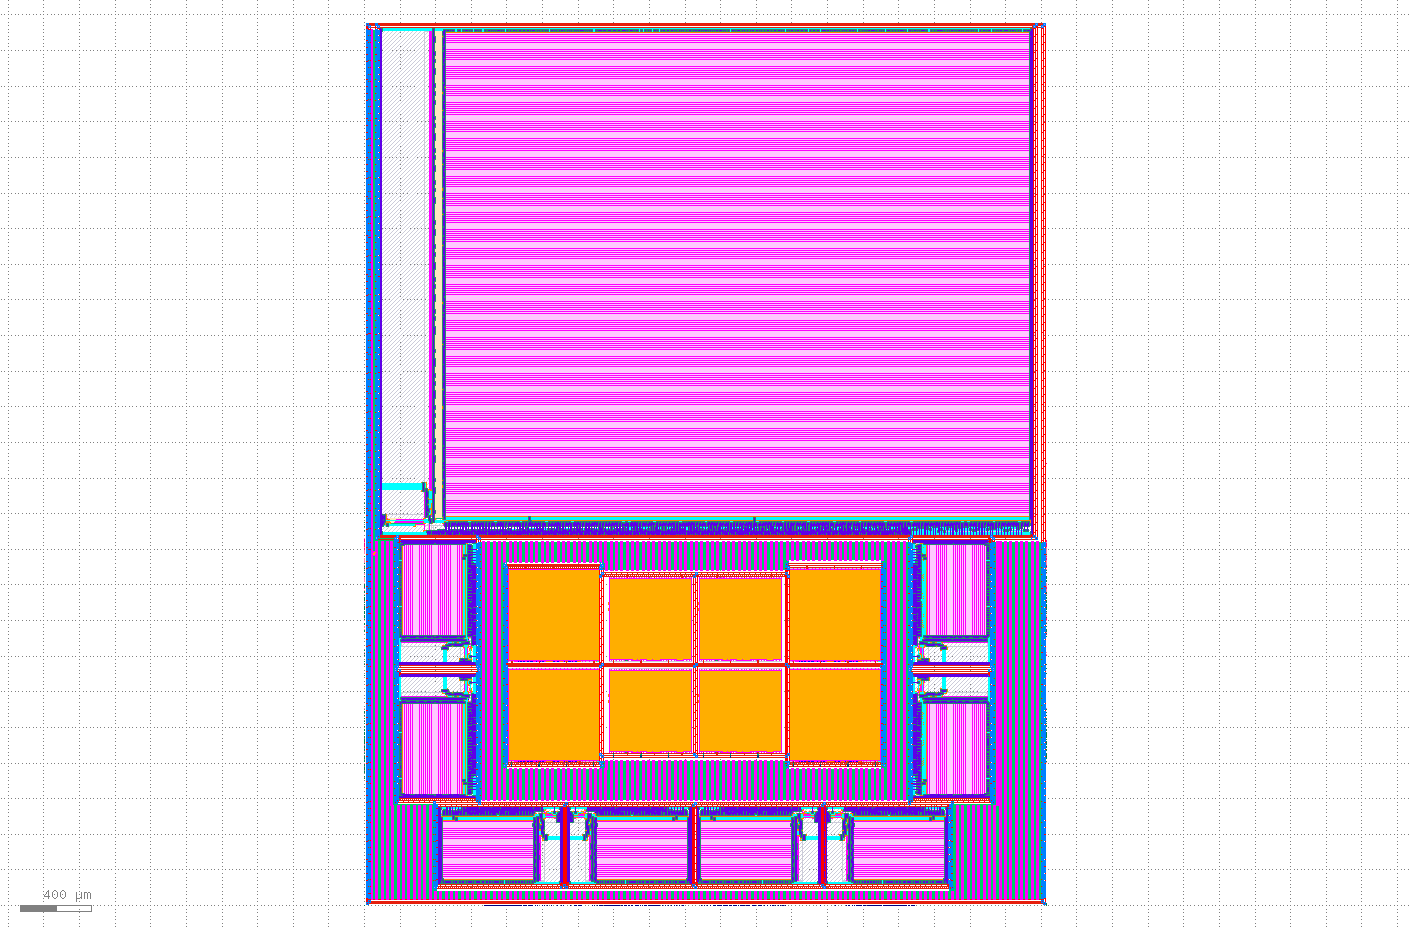
\includegraphics[width = 0.8\linewidth]{./ASIC/FP.png}
  \caption{Floorplan of Design}
  %\label{fig:Intro:flow}
\end{figure}

\subsection{Placements}
In the Placements and Routeing stage, convert the gate-level netlist produced during synthesis into a physical design. Placement involves placing all macros and cells into a specific and predefined space. It is done in three phases.
\begin{itemize}
\item Pre-placement optimizations are performed before placements and contain downsizing of the cells. It places the standard cells to optimize timing and congestion but not take into account overlapping prevention
\item In placement optimization, perform cell bypassing, gate duplication, and buffer insertion. It includes legalizing placement and eliminating overlap problems in the closest available space.
\item Post-placement optimization fixes set up and hold violations and are based on global routing. The clock consideration till the stage was ideal, and hence with clock skew, a post-placement optimization after CTS optimization is required.
\end{itemize}

\subsection{Clock Tree Synthesis}
Clock tree synthesis creates a balanced buffer tree in all high fanout clock nets to avoid violations regarding clock skew, max transition time, capacitance, and setup and hold times. This process includes 3 phases.
\begin{itemize}
\item Pre-CTS: The first step in the physical design is floor-planning. However, it can be manual by placing blocks. Accordingly, it's good to let the tool decide on a floor plan for you, and later, based on the analysis, Pre-CTS can instruct a proper floor plan. All the wire load models are removed before the placement, and absolute RC values from Virtual Route are considered to calculate timings. It performs different optimization at different stages. The downsizing of the cells is accomplished in Pre-placement optimizations. While at the time of placement optimization, cell bypassing, gate duplication, and buffer insertion. Post-placement optimization aims to fix setup and hold violations after the global routing. The clock is considered ideal till the stage.
\item CTS: The analysis used an ideal clock with zero skews. The software uses the FE-CTS commands to complete clock tree synthesis. In this mode, if present, the FE-CTS specification file is translated into a CCOpt clock tree specification Tcl script, and the clock tree synthesis is performed using the CCOpt engine.
\item Post-CTS: After successfully implementing clock tree synthesis in the design, we need to verify the design rule violations and the hold time. The command optDesign post-CTS will fix the error. The detailed routing for all the nets is performed.
\end{itemize}
\subsection{Routing}
Routing is about interconnecting the pins as per the netlist. This takes place in 2 phases.
\begin{itemize}
\item Global Routing: A loose route is generated for each net with estimated values in this type of routing. Global routing is further divided into Line Routing and Maze Routing.
\item Detailed Routing: In detailed routing, the actual geometry layout of each net is calculated, i.e., substantial delays of wire are calculated. Several optimizations like Timing optimization can obtain the exact delays, CTS, etc.
\end{itemize}

\subsection{Static timing analysis}
Static timing analysis is an integral part of Placement, Clock Synthesis, and Routing. A wire load model cannot guarantee accurate analysis and timing constraints. The difference between the accuracy of the analysis by both the tools can be examined when we use the parasitic extracted after the Place and Route. The buffers are used to improve the analysis and avoid violations.

\begin{figure}[h]
  \centering
  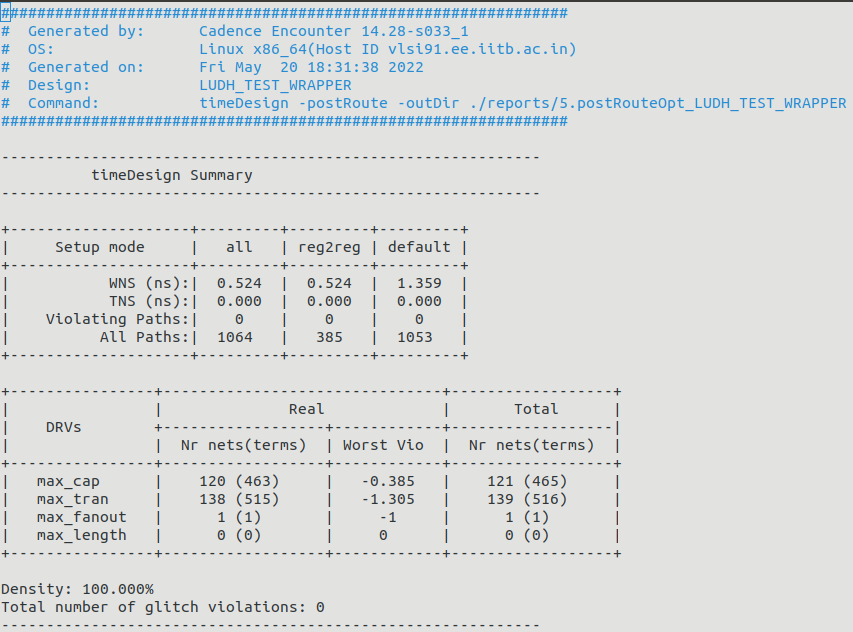
\includegraphics[width = 0.8\linewidth]{./ASIC/STA.png}
  \caption{Post Route QoR report}
  %\label{fig:Intro:flow}
\end{figure}

\subsection{Physical Verification}
Physical verification ensures a design's layout works as intended and does not violate the design constraints provided by the foundries. The increase in complex design with shrinking process geometries needs highly productive physical verification. 

\begin{itemize}
\item Antenna Rule Check is includes the maximum tolerance for the ratio of a metal line area to the area of connected gates.
\item Connectivity Checks is the Automated routing tools fail to check using connecting checks. This is a generic check.
\item Design rule checking (DRC) verifies if a chip layout satisfies the rules defined by the manufacturer. Each semiconductor process has its own set of rules, and we need to ensure sufficient margins so that normal variability in the process will not fail the chip.Geometry check is more like overlapping of cells, Same net, loop formation, etc. checks are done using geometry Check 
\item Layout vs. Synthesis (LVS) verifies if the generated structure is functionally the same as the schematic/netlist of the design we synthesized. It checks if we have transferred the geometry into the layout correctly. There should not be any missing nets or ports, or there should not be any shorts. In the case of semi-custom design, we do not have any schematic; hence we need to create a spice netlist to verify it with our generated layout.
\end{itemize}

\begin{figure}
  \begin{subfigure}{.5\textwidth}
    \centering
    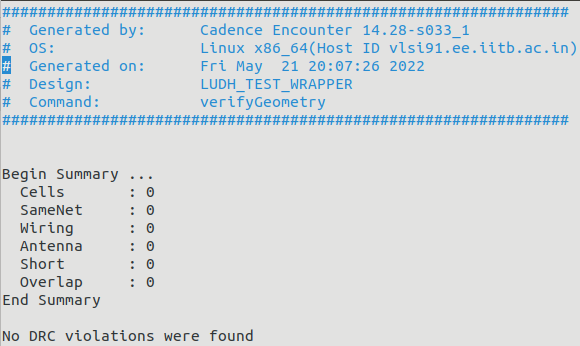
\includegraphics[width=.9\linewidth]{./ASIC/DRC.png}
    \caption{DRC Report}
  %	\label{fig:sfig1}
    \end{subfigure}%
    \begin{subfigure}{.5\textwidth}
    \centering
    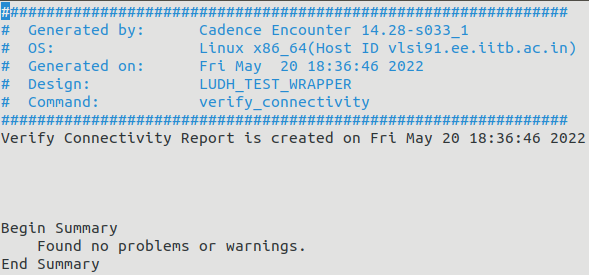
\includegraphics[width=.9\linewidth]{./ASIC/Connectivity.png}
    \caption{Connectivity}
  %	\label{fig:sfig2}
    \end{subfigure}
    \begin{subfigure}{.5\textwidth}
      \centering
      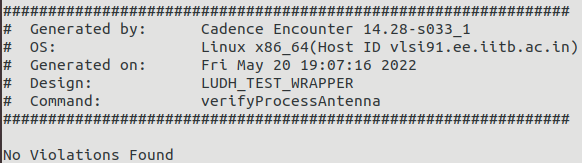
\includegraphics[width=.9\linewidth]{./ASIC/ProcessAntenna.png}
      \caption{Process Antenna Report}
    %	\label{fig:sfig2}
      \end{subfigure}
      \begin{subfigure}{.5\textwidth}
        \centering
        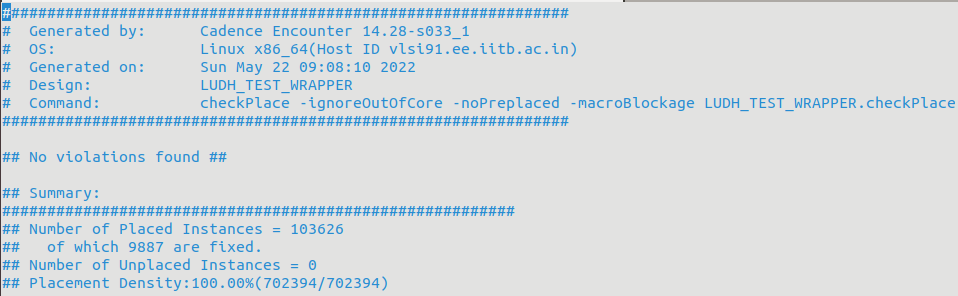
\includegraphics[width=.9\linewidth]{./ASIC/Placement.png}
        \caption{Placement Report}
      %	\label{fig:sfig2}
        \end{subfigure}  
      \begin{subfigure}{.5\textwidth}
        \centering
        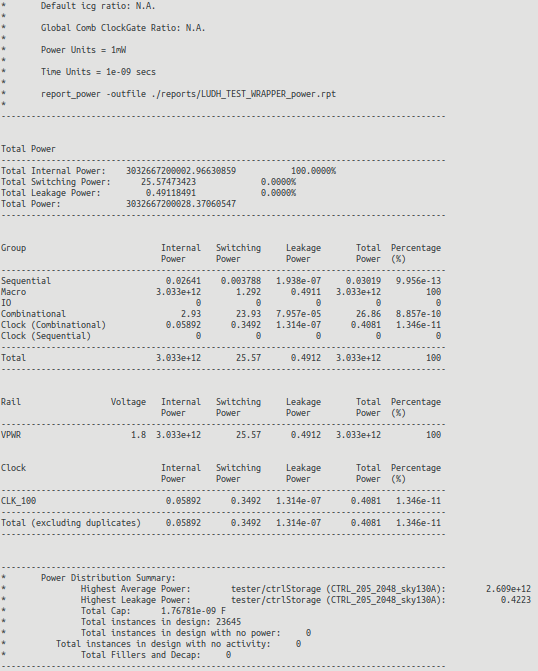
\includegraphics[width=.9\linewidth]{./ASIC/POWER.png}
        \caption{Power Report}
      %	\label{fig:sfig2}
        \end{subfigure}
    \caption{DRC, Placement, Connectivity, Antenna Check report and Power Summarry}
  %  \label{fig:fig}
  \end{figure}


The proper sign-off tools, Cadence ASSURA or Mentor Graphics Calibre, files are not provided by Skywater 130 nm Foundry. Generic Tests are successfully passed in Cadene Soc Encounter.

